\documentclass[12pt]{article}
\usepackage[utf8]{inputenc}
\usepackage{float}
\usepackage{amsmath}


\usepackage[hmargin=3cm,vmargin=6.0cm]{geometry}
%\topmargin=0cm
\topmargin=-2cm
\addtolength{\textheight}{6.5cm}
\addtolength{\textwidth}{2.0cm}
%\setlength{\leftmargin}{-5cm}
\setlength{\oddsidemargin}{0.0cm}
\setlength{\evensidemargin}{0.0cm}

%misc libraries goes here
\usepackage{tikz}
\usetikzlibrary{automata,positioning}

\begin{document}

\section*{Student Information } 
%Write your full name and id number between the colon and newline
%Put one empty space character after colon and before newline
Full Name : Kadir CETINKAYA \\
Id Number : 2036457 \\

% Write your answers below the section tags
\section*{Answer 1}

\subsection*{a.}
%$a\{a,c\}^*b\{a,c\}^*b\{a,c\}^*cc$
$a(a+c)^*b(a+c)^*b(a+c)^*cc$

\subsection*{b.}
%$\{(\{b,c\}\{b,c\})^*a\{b,c\}(\{b,c\}\{b,c\})^*\} \cup \{\{b,c\}(\{b,c\}\{b,c\})^*a(\{b,c\}\{b,c\})^*\}$
$(((b+c)(b+c))^*a(b+c)((b+c)(b+c))^*)+((b+c)((b+c)(b+c))^*a((b+c)(b+c))^*)$
\subsection*{c.}
$a^*(b^*baa^*b^*baa^*)^*b^*$

\section*{Answer 2}

\subsection*{a.}
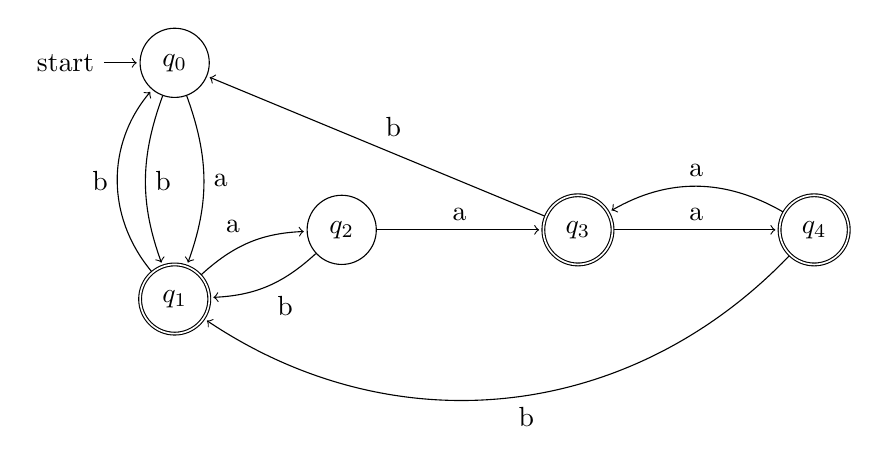
\begin{tikzpicture}[shorten >=1pt,node distance=3cm,on grid,auto]
\node[state,initial] (q_0) {$q_0$};
\node[state,accepting] (q_1) [below=of q_0] {$q_1$};
\node[state] (q_2) [below right=of q_0] {$q_2$};
\node[state,accepting](q_3) [right=of q_2] {$q_3$};
\node[state,accepting](q_4) [right=of q_3] {$q_4$};
\path[->]
	(q_0) edge [bend left=20]  node {a} (q_1)
	(q_0) edge [bend right=20] node {b} (q_1)
	(q_1) edge [bend left=40] node {b} (q_0)
	(q_1) edge [bend left=20] node {a} (q_2)
	(q_2) edge node {a} (q_3)
	(q_2) edge [bend left=20] node {b} (q_1)
	(q_3) edge node {a} (q_4)
	(q_3) edge node [swap] {b} (q_0)
	(q_4) edge [bend right] node [swap] {a} (q_3)
	(q_4) edge [bend left=40] node {b} (q_1);
\end{tikzpicture}

\subsection*{b.}
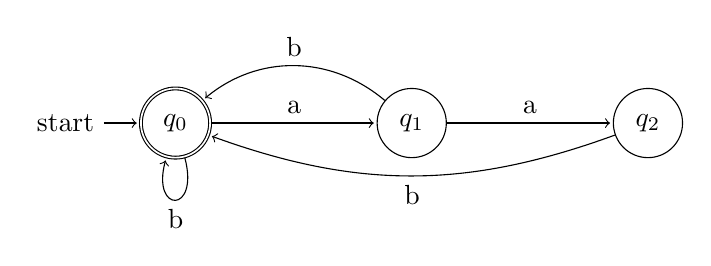
\begin{tikzpicture}[shorten >=1pt,node distance=3cm,on grid,auto]
\node[state,initial, accepting] (q_0) {$q_0$};
\node[state] (q_1) [right=of q_0] {$q_1$};
\node[state] (q_2) [right=of q_1] {$q_2$};
\path[->]
	(q_0) edge [loop below]  node {b} ()
	(q_0) edge node {a} (q_1)
	(q_1) edge [bend right=40] node [swap] {b} (q_0)
	(q_1) edge node {a} (q_2)
	(q_2) edge [bend left=20] node {b} (q_0);
\end{tikzpicture}

\section*{Answer 3}
Let us examine the case where $L_i=\{a^ib^i\}, i\in N$ and the alphabet used is $\Sigma = \{a,b\}$.
Clearly each $L_i$ is a regular language, since they only consist of one word. Their union is \\
$L=\cup_{i=0}^{\infty}L_i=\{a^ib^i|i\in N\}$. According to Pumping lemma $\exists p \ge 1$ s.t. 
$\forall w\in L, |w|\ge p$ can be written as $w=xyz$, with the following properties:

\def\labelitemi{-}
\begin{itemize}
	\item $|y|\ge 1$
	\item $|xy|\le p$
	\item $\forall i\ge 0, xy^iz\in L$
\end{itemize}

So let us choose $w$ as $w=a^pb^p$, since that $p$ exists according to lemma, we can split the $w$
into three parts, since $|xy|\le p$ and $|y|\ge 1$ and $w$ contains $p$ $a$'s as prefix, $y$
contains at least one $a$. According to third property we should have $xy^0z\in L$, but that's
clearly not true since $L$ contains only words containing same amount of $a$'s and $b$'s whereas $xy^0z$
contains absolutely less $a$'s then $b$'s. So, $L$ is not a regular language. Therefore, despite
$L$ is countably infinite union of regular languages, itself is not a regular language so the claim
is false.



\section*{Answer 4}
Let $L=\{a^ib^jc^{2j} | i\ge 0,j\ge 0\}$ and $w\in L$, according to pumping lemma $\exists p\ge 1$ s.t.\\
$\forall w\in L,\{a^ib^jc^{2j} | i\ge 0,j\ge 0\} |w|\ge p$ can be written as $w=xyz$, with the 
following properties:
\def\labelitemi{-}
\begin{itemize}
	\item $|y|\ge 1$
	\item $|xy|\le p$
	\item $\forall i\ge 0, xy^iz\in L$
\end{itemize}

If $p=1$, it is clear that string $w=b^1c^2\in L$, when split into $w=xyz$, $xy=y=b$ by the pumping lemma
and $xy^0z$ definitely would not be in $L$, since amount of $b$'s would be $0$ while amount of $c$'s is still $2$.
Contradiction.

If $p>1$ let us choose $w$ as $w=b^{j_0}c^{2j_0}$ where $j_0=p$ into $w=xyz$, since we assume $p>1$ and by
the pumping lemma $y$ contains at least one $b$ and definitely no $c$. So, $xy^0z\notin L$ since amount of
$b$'s is less than $j_0$ whereas there are exactly $2j_0$ of $c$'s. Contradiction.

Since we got a contradiction for any choice of $p$, $L$ is not regular.



\section*{Answer 5}
Let us choose 2 regular languages $L_1$ and $L_2$, with correspoding deterministic finite automatas\\
$M_1=(Q_1, \Sigma_1, \Delta_1, s_1, F_1)$ and $M_2=(Q_2, \Sigma_2, \Delta_2, s_2, F_2)$.\\
Now let us create a new finite automata $M=(Q, \Sigma, \Delta, s, F)$, where $Q=(Q_1\times Q_2)$,
$\Sigma =\Sigma_1 \cup \Sigma_2$,\\
$\Delta =\{((q_1,q_2), \sigma, (q_1', q_2'))| \sigma \in \Sigma, (q_1,\sigma,q_1')\in \Delta_1, (q_2,\sigma,q_2')\in \Delta_2\}$,
$s=(s_1,s_2)$,\\ $F=\{(q_1, q_2) | q_1\in F_1, q_2\in Q_2-F_2\}$. Now from that definition it is easy
to see that $(p,q)$ is an accepting state for $M$ iff $p$ is an accepting state for $M_1$ and $q$ is
a nonaccepting state for $M_2$. Also $(p,q)$ is an inital state iff $p$ is inital state of $M_1$ and
$q$ is inital state of $M_2$. Also transitions are done for the first element of the state tuple
according to $\Delta_1$ and for the second element of the state tuple according to $\Delta_2$.

\begin{itemize}
	\item Claim I: $L(M)\subseteq L(M_1)-L(M_2)$\\
		Let $x\in L(M)$, since DFA $M$ accepts that string, state must be of the form $(p,q)$
		which implies by the construction of $M$, DFA $M_1$ would be in state $p$ and DFA $M_2$
		would be in state $q$, also by the construction of $M$ we know that $p$ is an accepting
		state for $M_1$ whereas $q$ is not an accepting state for $M_2$. So, $M_1$ accepts $x$
		but $M_2$ does not. Therefore $x\in L(M_1) \wedge x\notin L(M_2)\rightarrow x\in L(M_1)-L(M_2)$
		So our claim holds.
	\item Claim II: $L(M_1)-L(M_2)\subseteq L(M)$\\
		Let $x\in L(M_1)-L(M_2)\rightarrow x\in L(M_1) \wedge x\notin L(M_2)$, this implies $M_1$
		accepts $x$ whereas $M_2$ does not. So $M_1$ must be in an accepting state say $p$ while
		$M_2$ must be in a nonaccepting state say $q$. So if we given $x$ to DFA $M$ it would be
		in state $(p,q)$ which is an accepting state for $M$ since $p$ is an accepting state for
		$M_1$ and $q$ is a nonaccepting state for $M_2$ by construction. Therefore
		$x\in L(M_1)-L(M_2)\rightarrow x\in L(M)$. So our claim holds.
	\item So by Claim I and II it is easy to see that $L(M)=L(M_1)-L(M_2)=L_1-L_2$ and since $M$
		is a DFA, $L(M)$ is a regular language. Therefore regular languages are closed under set
		difference.
\end{itemize}

\section*{Answer 6}
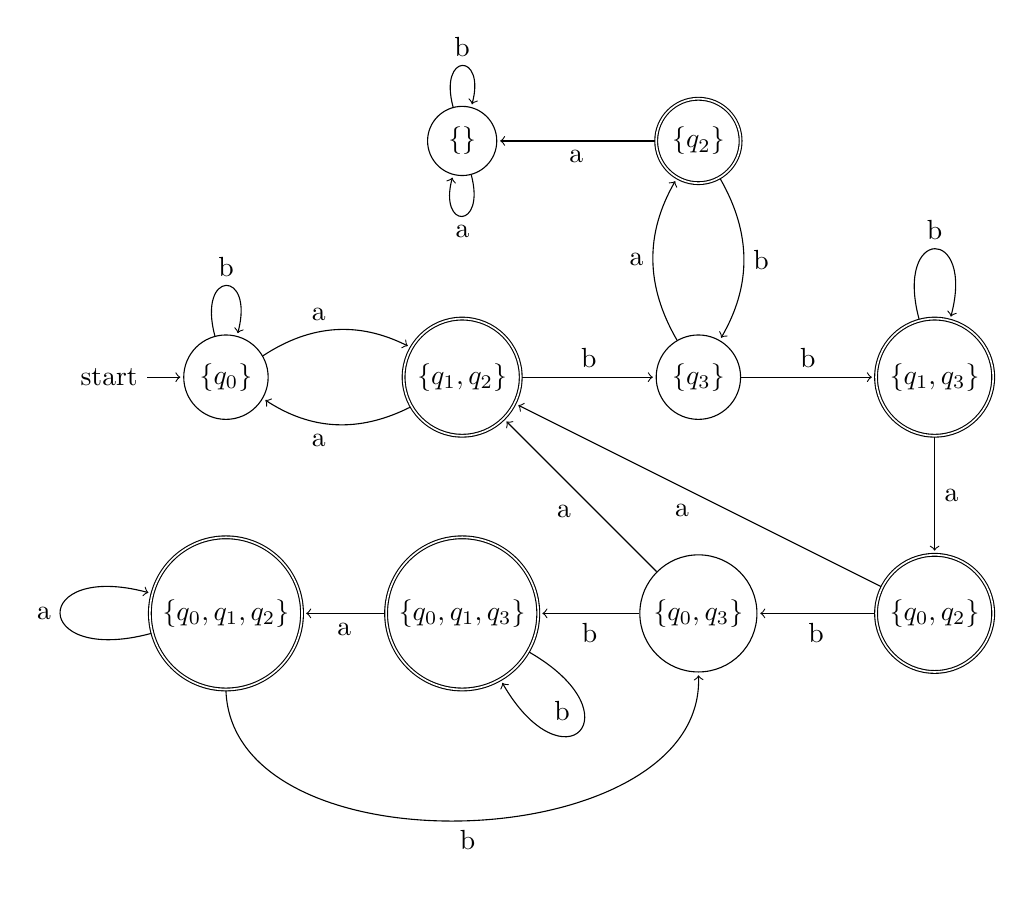
\begin{tikzpicture}[shorten >=1pt,node distance=3cm,on grid,auto]
	\node[state,initial] (q0) {$\{q_0\}$};
	\node[state, accepting] (q1) [right=of q0] {$\{q_1,q_2\}$};
	\node[state] (q2) [right=of q1] {$\{q_3\}$};
	\node[state, accepting] (q3) [above=of q2] {$\{q_2\}$};
	\node[state, accepting] (q4) [right=of q2] {$\{q_1,q_3\}$};
	\node[state, accepting] (q5) [below=of q4] {$\{q_0,q_2\}$};
	\node[state] (q6) [left=of q5] {$\{q_0,q_3\}$};
	\node[state, accepting] (q7) [left=of q6] {$\{q_0,q_1,q_3\}$};
	\node[state, accepting] (q8) [left=of q7] {$\{q_0,q_1,q_2\}$};
	\node[state] (q9) [left=of q3] {$\{\}$};
\path[->]
	(q0) edge [loop above]  node {b} ()
		 edge [bend left] node {a} (q1)
	(q1) edge node {b} (q2)
		 edge [bend left] node {a} (q0)
	(q2) edge [bend left] node {a} (q3)
		 edge node {b} (q4)
	(q3) edge [bend left] node {b} (q2)
		 edge node {a} (q9)
	(q4) edge [loop above] node {b} ()
		 edge node {a} (q5)
	(q5) edge node {a} (q1)
		 edge node {b} (q6)
	(q6) edge node {a} (q1)
		 edge node {b} (q7)
	(q7) edge [out=330,in=300,looseness=8,loop] node [swap] {b} ()
		 edge node {a} (q8)
	(q8) edge [loop left] node {a} ()
		 edge [bend right=90] node [swap] {b} (q6)
	(q9) edge [loop below] node {a} ()
		 edge [loop above] node {b} ();
\end{tikzpicture}

The correspondence is shown in the node names, as they are subsets of the states of the
given NFA. Also the constructed DFA is minimal, since for every state $q$ in it there exists
a word $w$ such that $(\{q_0\}, w) \vdash_M^* (q, e)$ which implies there is no unreachable
state and also for every state pair $(p,q)$ there exists a word $w$ such that,
$(p,w) \vdash_M^* (p',e)$, $(q,w) \vdash_M^* (q',e)$ where $(p'$ is an accepting state and
$q'$ is a nonaccepting state $)$ or $(p'$ is a nonaccepting state and $q'$ is an accepting
state $)$ which implies every two state is distinguishable from each other.



\end{document}

​

